\section{Proposed NeST-Com Framework}
\subsection{Next-Scale Representation and Digital Frame}
We transmit $x\in[0,1]^{256\times256\times3}$ over complex AWGN,
\begin{equation}
 y=s+n,\quad n\sim\mathcal{CN}(0,\sigma^2 I_N),\quad
 \mathrm{SNR}=10\log_{10}(E_s/\sigma^2),
 \label{eq:channel}
\end{equation}
using $N$ complex symbols per image and nominal $E_s=2$. TX selects a frozen policy for the channel SNR; RX uses the true noise variance for LLRs. Digital constellations have average energy two without per-frame renormalization. Continuous JSCC data are normalized per image to average energy two, with required Swin side information paid within $N$. A 12-bit profile ID, CRC16, and terminated rate-1/2 convolutional code occupy 68 rotated-BPSK symbols $\{\pm(1+j)\}$. The remaining $N-68$ symbols carry the LDPC-coded body. After rate matching, a public frame-dependent scrambling mask is applied before QAM modulation and reversed at the receiver before LDPC decoding. The paid profile identifies the actual endpoint and MCS. Our main budget is $N=1024$; the reduced-budget experiment uses $N=512$ without increasing $E_s$.

The frozen VAR tokenizer produces ten residual token maps $q_s$, with side lengths $(1,2,3,4,5,6,8,10,13,16)$ and a 4096-entry codebook~\cite{var}. Let $h_s$ denote the side length, $L_s=h_s^2$ the number of positions, and $C_s$ the scale-dependent codebook lookup, resizing, and residual transform. Complete coarse maps span the whole latent grid after resizing; the sum $f_q=\sum_s C_s(q_s)$ accumulates their residual refinements. Image decoder $\Dc$ is adapted on 20\,000 ImageNet training images using continuous, fully quantized, and prefix-completion-interpolated latents, then fixed. NeST-Com uses null-class conditioning. Its frozen VAR-d16 next-scale prior factorizes~\cite{var} as
\begin{equation}
 p_\theta(q_s\mid q_{<s})=\prod_{i=1}^{L_s}p_\theta(q_{s,i}\mid q_{<s}),
 \label{eq:prior}
\end{equation}
All positions in a scale thus obtain coding probabilities from the same complete coarse maps. Both terminals construct the same integer cumulative distribution functions (CDFs), with total frequency $2^{24}$, for arithmetic coding~\cite{arithmetic} of a within-scale subset (Fig.~\ref{fig:system}; Supplement~S1.1).

\begin{figure*}[t]
\centering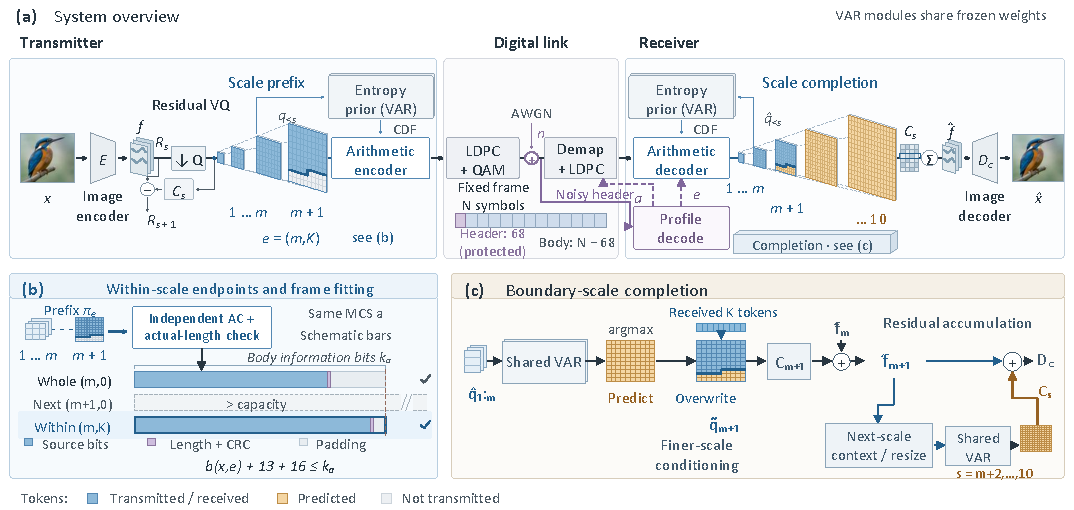
\includegraphics[width=\textwidth]{figure1.pdf}
\caption{NeST-Com: (a) The protected profile and body share the fixed noisy frame; both terminals reconstruct coding probabilities from the shared frozen VAR and known coarse tokens. (b) Independently terminated within-scale prefixes fit the body information capacity; bars are schematic for the same MCS. (c) Received tokens overwrite boundary predictions, and the merged map updates the residual latent and finer-scale context while unreceived positions retain their coarse-conditioned predictions.}
\label{fig:system}
\end{figure*}

\subsection{Within-Scale Endpoints and Actual-Length Fitting}
An endpoint $e=(m,K)$ retains complete coarse maps and $K$ raster-ordered positions from the next map:
\begin{equation}
 \pi_e=(q_1,\ldots,q_m,q_{m+1,1:K}).
 \label{eq:prefix}
\end{equation}
For $K=0$, the boundary tail is absent. WHOLE permits $K=0$ for $m=4,\ldots,10$. PARTIAL adds
$K\in\{\lfloor L_{m+1}/4\rfloor,\allowbreak\lfloor L_{m+1}/2\rfloor,\allowbreak\lfloor3L_{m+1}/4\rfloor\}$ for $m=4,\ldots,9$, giving 25 endpoints in total. $(10,0)$ is the full representation.

For MCS $a=(M,r)$, the coded body has $n_a=(N-68)\log_2M$ bits and information length $k_a=\lfloor rn_a\rfloor$. With actual terminated arithmetic length $b(x,e)$,
\begin{equation}
 b(x,e)+29\leq k_a,\qquad \eta(x,e)=\frac{b(x,e)}{k_a-29}.
 \label{eq:budget}
\end{equation}
The endpoint specifies retained source tokens; its actual terminated length determines frame feasibility. The 29 bits comprise the 13-bit length field and CRC16; unused information positions are zero-padded before 5G NR LDPC coding, rate matching~\cite{nr}, and QAM. Thus $\eta$ measures source-bit capacity utilization, not total over-the-air efficiency.

Offline calibration selects a target endpoint and MCS separately for each budget and SNR on an independent image set. It maximizes source/reconstruction DINOv2 cosine~\cite{dinov2}, averaged first over channel realizations and then equally over sources. The selected policy is frozen for testing; candidate pools and screening rules are given in Supplement~S1; targets and MCSs are in S1.1.

Candidate prefixes share one scale-wise probability and incremental arithmetic-coding traversal. Non-mutating finalization produces an independently terminated stream at each legal endpoint; no stream is cut from a longer one. With the calibrated MCS fixed, TX checks endpoints no longer than the target in decreasing token count down to $(4,0)$ and selects the first satisfying~\eqref{eq:budget}. This retains the most tokens among feasible candidates without assuming monotone code lengths or optimizing per-image distortion. If none fits, a paid NULL profile and short payload occupy the full frame and yield gray. Both budgets support this behavior; the versioned N1024 extension preserves normal paths (Supplement~S7). Historical N1024 evaluations used error-on-no-fit and never encountered that case.

\ifCLASSOPTIONonecolumn\else\begin{figure*}[t]
\centering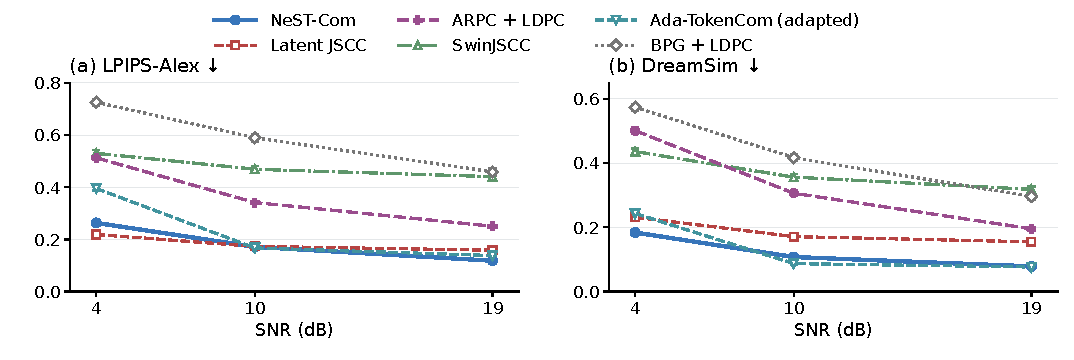
\includegraphics[width=\textwidth]{figure2.pdf}
\caption{Source-referenced perceptual distances on common500 at $N=1024$. Points and error bars are equal-source means and pointwise 95\% source-bootstrap intervals after averaging three channel outcomes per source. Lower LPIPS-Alex and DreamSim are favorable. Ada denotes the predicted-class, fixed-frame adaptation.}
\label{fig:performance}
\end{figure*}
\fi
\subsection{Prefix-Constrained Reconstruction}
Invalid profile CRC/catalogue, body CRC, declared length, known padding, or arithmetic parsing produces a fixed gray image; so does a valid NULL reception. Otherwise, RX decodes the prefix using CDFs rebuilt from received complete coarse maps. It predicts the boundary map by VAR argmax conditioned on those maps, then applies known-token overwrite~\cite{var}:
\begin{equation}
 \tilde q_{m+1,i}=\begin{cases}\hat q_{m+1,i},&i\leq K,\\q^{\mathrm{pred}}_{m+1,i},&i>K.\end{cases}
 \label{eq:overwrite}
\end{equation}
Unreceived boundary positions retain their coarse-conditioned prediction. Received boundary tokens serve two roles: they correct the residual representation and, through the merged boundary map, condition the prediction of finer scales. Complete received maps remain unchanged; subsequent maps are generated from this updated context. Reconstruction is
\begin{equation}
 \hat x=\Dc\!\left(\sum_{s=1}^{10}C_s(\tilde q_s)\right).
 \label{eq:reconstruction}
\end{equation}
At the final scale, overwrite changes the residual contribution without any subsequent propagation.
